\chapter{Design Optimization}
\label{chapter-six}

Design optimization is a wide field that encompasses methods generally falling
into two categories: local gradient-based optimization, and heuristic global
optimization.  Local gradient-based optimization techniques focus on the
determining an optimality condition by evaluating a function and its gradients.
Provided certain conditions are met, it can be proven that the optimization
procedure will find a local minimum or maximum on a bounded domain.  Examples of
local gradient-based optimization methods include
steepest-descent\cite{fletcher1963rapidly}, sequential quadratic programming
(SQP)\cite{SNOPT-alg}, as well as an interesting method that converts a
constrained optimization problem into an unconstrained on by employing the
Kreisselmeier-Steinhauser function\cite{wrenn1989indirect}.  A heuristic global
optimization seeks to find the global extrema of a function.  Although these
methods are powerful, because of their heuristic nature they are not guaranteed
to find the absolute optimum condition and are not the focus this research.

In the field of optimization, the function of interest is referred to as the
``cost function'' or ``objective function''.  Optimization methods seek to
minimize this function; therefore, if the intent is to find the maximum value
of the function, it should be formulated as the negative of the original.  This
section focuses on geometry and test conditions for the optimization, the
implementation of the cost function components and design variables used in the
optimization, as well as the interface to the optimizer that is used.

\section{Integrated Quantities of Interest}

The primary objective of this optimization is to explore the effects of the plume
from the annular jet interacting with the bow shock.  Rather than focus on the
net force contribution of this annular jet geometry to drag, as was previously
investigated by Gnoffo et. al \cite{gnoffo2016tapping}, the primary objective of
this study is to efficiently cool the surface of the vehicle with minimal mass
added to the vehicle.  Since only inviscid flow was done in this study, and the
root-mean-square (RMS) of surface temperature is taken as an analog to the
surface heating rate.  Likewise, the massflow rate through nozzle plenum
boundary is taken as an analog to the addition of mass to the vehicle.

The RMS of surface temperature is defined as
%------------------------------------------------------------------------------%
\begin{equation}
  T_{RMS} =
  \sqrt{
    \frac{\sum_{i}^{N_{faces}}\left( T_{RMS} A_i \right)^2}
       {\sum_{i}^{N_{faces}}\left( A_i \right)^2}
     }
  \label{tt-rms-def}
\end{equation}
%------------------------------------------------------------------------------%
The area-weighted RMS of surface temperature was chosen over a simple
area-weighted average of surface temperature, because the temperatures on the
vehicle forebody are likely non-uniform, and there are regions of very high
temperature near the stagnation region of a vehicle forebody in hypersonic
flows.  Squaring of temperature in the RMS will give greater weight to the
these high-temperature regions in the design, as these are the in the most
danger of burn-through.
%------------------------------------------------------------------------------%
\begin{figure}[h]
  \centering
	\begin{subfigure}[b]{0.4\textwidth}
    \centering
    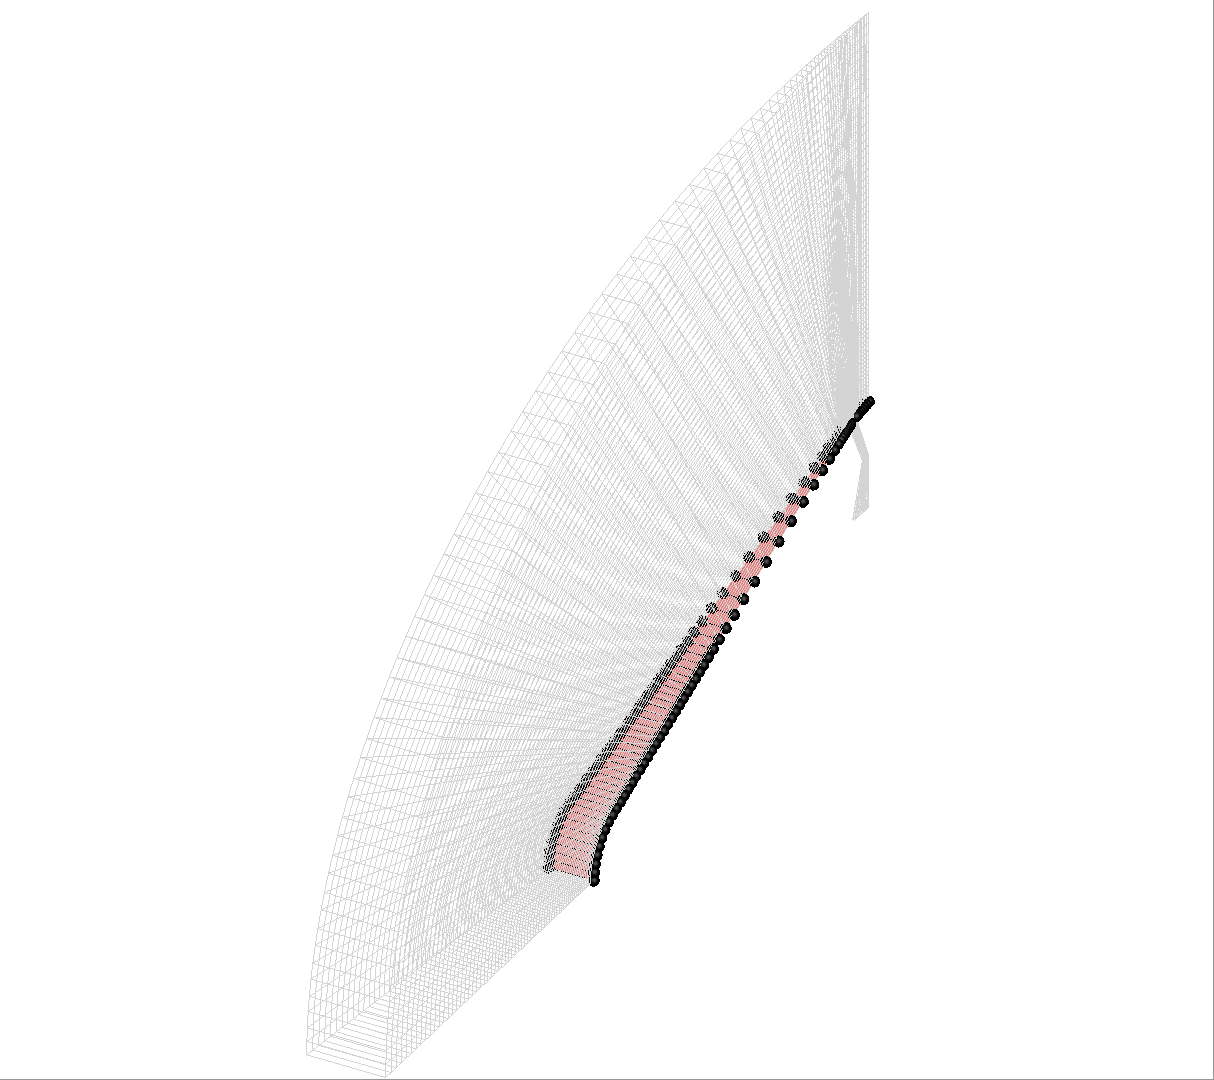
\includegraphics[width=\textwidth]{figures/surface2.png}
    \caption{$T_{RMS}$ Integrated Area}
    \label{fig:t-rms-area}
  \end{subfigure}
	\begin{subfigure}[b]{0.4\textwidth}
    \centering
    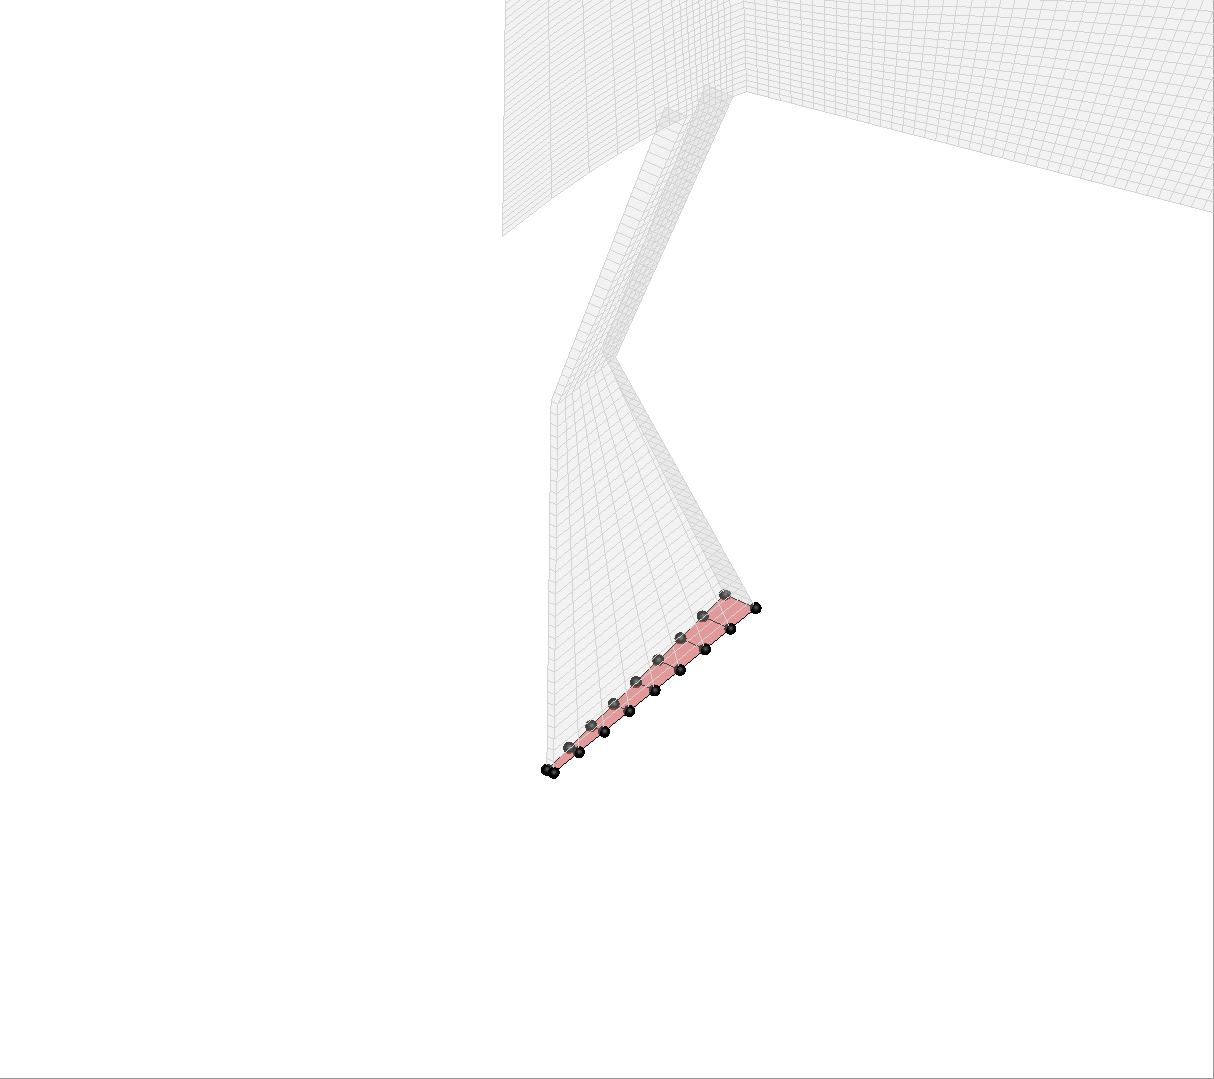
\includegraphics[width=\textwidth]{figures/plenum_bc.png}
    \caption{Mass Flow Rate Integrated Area}
    \label{fig:plenum-face}
  \end{subfigure}
\end{figure}
%------------------------------------------------------------------------------%

The mass flow rate, $\massflow$,
through the area outlined in \fref{fig:plenum-face} is computed as
%------------------------------------------------------------------------------%
\begin{equation}
  \massflow = \sum_{i}^{N_{faces}}\left( \rho_i \overline{U} A \right)
  \label{mass-flow-eqn}
\end{equation}
%------------------------------------------------------------------------------%
and is used a metric for the amount of propellent that is required to be carried
by the vehicle for blowing.  Again, for the purposes of this demonstration
problem, a lower mass flow rate at the plenum is equated to less total vehicle
mass.

\section{Composite Cost Function Definition and Components}
\label{cost-func-components}

The cost function (or objective function) as formulated in FUN3D is a composite,
weighted function
%------------------------------------------------------------------------------%
\begin{equation}
  f = \sum_{j=1}^{N_{func}}w_j\left( C_j - C_{j^*} \right)^{p_j}
  \label{generic-cost-function}
\end{equation}
%------------------------------------------------------------------------------%
Where $w_j$, $C_{j^*}$, and $p_j$ are the weight, target, and power of cost
function component $j$.  $C_j$ is the component value, which is evaluated at
each flow solution.  For example, an optimization problem that seeks to minimize the
surface temperature RMS without decreasing the drag, the cost function is
defined as 
%------------------------------------------------------------------------------%
\begin{equation}
  f = w_1\left( T_{RMS} \right)^{2} + w_2\left( C_{D} - C_{D}^{*} \right)^2
  \label{cd-tt-cost-function}
\end{equation}
%------------------------------------------------------------------------------%
For this case the component weights must be determined heuristically, to normalize
the changes in drag coefficient, $C_D$, and surface temperature Root-Mean-Square
(RMS) $T_{RMS}$.  The terms in \eref{cd-tt-cost-function} are squared to provide
a convex design space.

\section{Design Variables}

The design variables for the optimization problem are the plenum total pressure,
$P_{p,o}$, plenum total temperature, $T_{p,o}$, and plenum ``fuel-air ratio'',
$\fa$.  These are provided explicitly in the optimization problem, and are used
to directly set the flow conditions on plenum face boundary condition in the
nozzle, shown in \fref{fig:plenum-face}.  For a reacting gas mixture, the
``fuel-air ratio'' specifies the mass fractions for two species leaving the
plenum.  For example, if an $H_2-N_2$ mixture is ejected from the annular
nozzle, the mass fractions of $H_2$ and $N_2$ are given by
%------------------------------------------------------------------------------%
\begin{equation}
  \begin{aligned}
    c_{H_2} &= \fa \\
    c_{N_2} &= 1 - \fa
  \end{aligned}
  \label{fuel-air-def}
\end{equation}
%------------------------------------------------------------------------------%
Thus, the ratio $\fa$ dictates the mass fractions for two species injected into
the domain via the plenum boundary.

\section{Obtaining Sensitivity Gradients for Design Variables}

The sensitivity gradients for the plenum design variables are easily obtained by
manipulating \eref{obj-function} to obtain
%------------------------------------------------------------------------------%
\begin{equation}
  \pd{L}{\md} = \pd{f}{\md} + \rtdiff{}{\md} \mathbf{\Lambda}
  \label{obj-linearization1}
\end{equation}
%------------------------------------------------------------------------------%
For the cost function components listed in \sref{cost-func-components}, there is
no direct dependence on the plenum design variables; thus,
\eref{obj-linearization1} can be reduced to
%------------------------------------------------------------------------------%
\begin{equation}
  \pd{L}{\md} = \rtdiff{}{\md} \mathbf{\Lambda}
  \label{obj-linearization2}
\end{equation}
%------------------------------------------------------------------------------%
Once the adjoint co-state variables $\mathbf{\Lambda}$ have been computed by
solving the adjoint equations (\eref{adjoint-main}) the sensitivity derivatives
of the cost function with respect to the plenum design variables are obtained by
evaluating relatively inexpensive matrix-vector products.

\section{Inverse Design Optimization}
\label{inv-design-opt}

The optimization procedure is done using the \textit{opt\_driver} utility in
FUN3D, which is a wrapper utility that executes the FUN3D flow solver, adjoint
solver, and optimization algorithm sequentially.  These steps are repeated until
a termination criterion is reached.  In practice, the termination of the
optimization occurs when the cost function reaches a tolerance of less that
$10^{-8}$, or when continuing towards the optimal condition would exceed the
prescribed upper or lower bounds of the design variables.

%------------------------------------------------------------------------------%
\begin{figure}[h]
  \centering
	\begin{subfigure}[b]{0.45\textwidth}
    \centering
    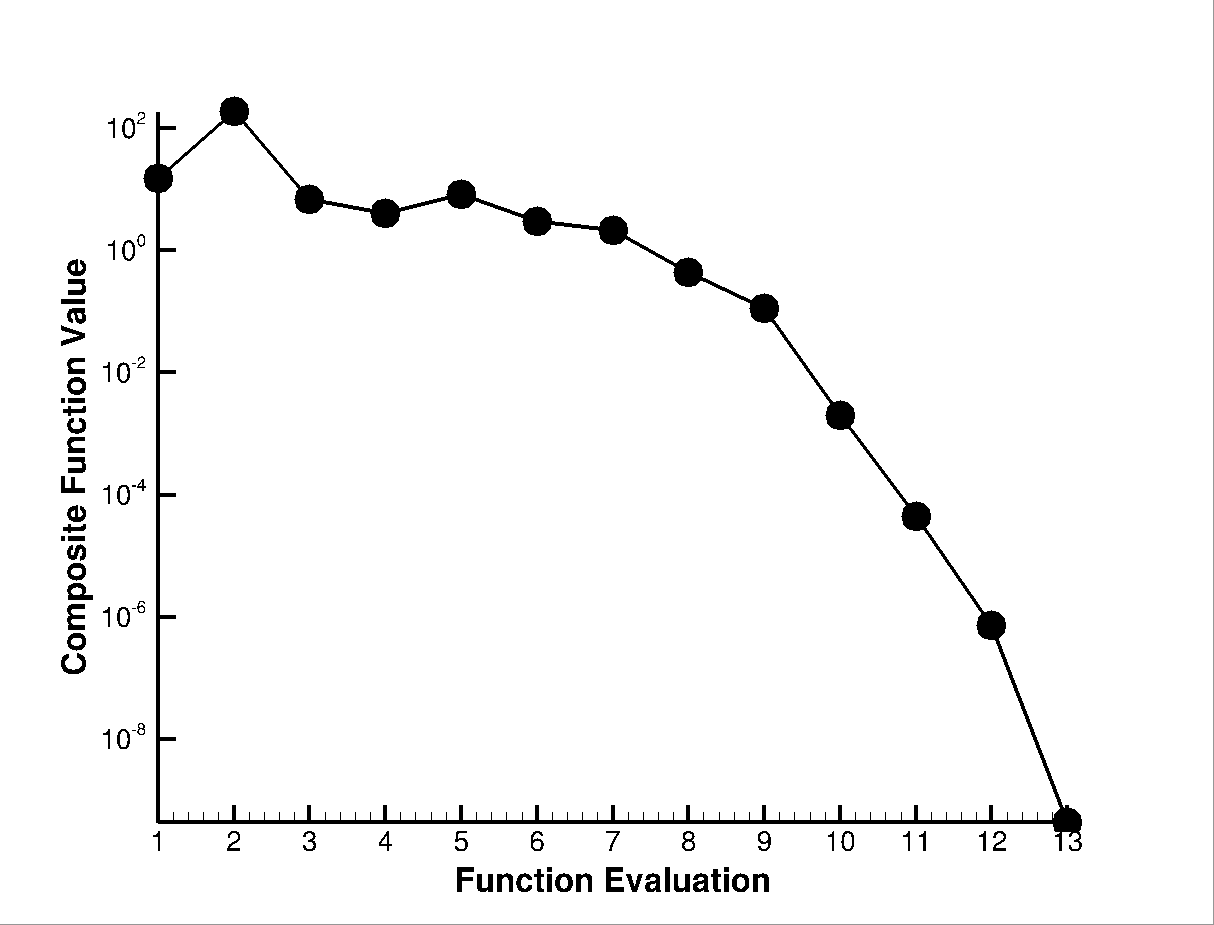
\includegraphics[width=\textwidth]{figures/1st-H2/cost_func.png}
    \caption{Composite Value}
    \label{fig:cost-func-1st-H2}
  \end{subfigure}
	\begin{subfigure}[b]{0.45\textwidth}
    \centering
    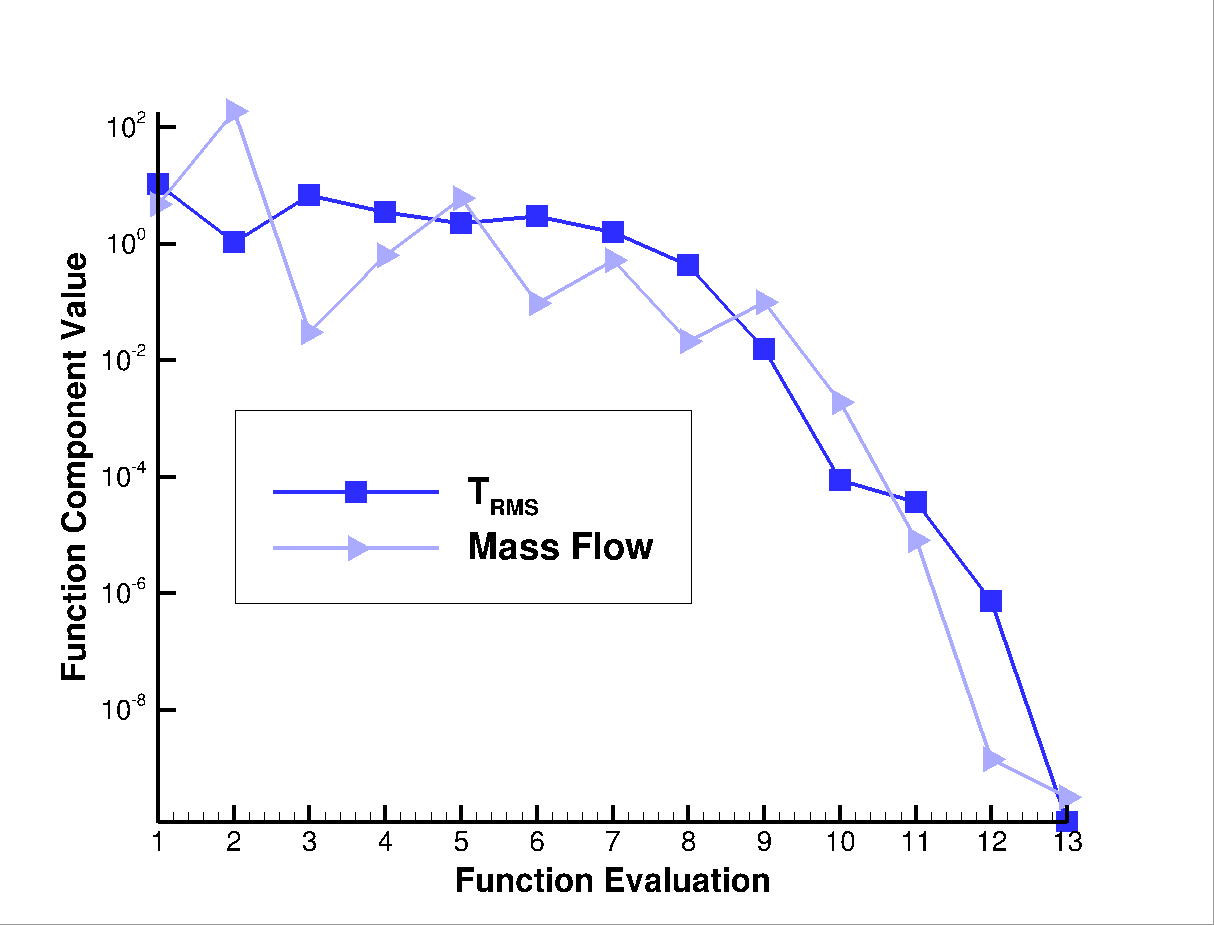
\includegraphics[width=\textwidth]{figures/1st-H2/func_components.png}
    \caption{Component Values}
    \label{fig:components-1st-H2}
  \end{subfigure}
  \caption{Cost Function and Component History}
\end{figure}
%------------------------------------------------------------------------------%
To demonstrate the inverse design capability of an adjoint-based design
optimization, targets of 2000 K for the surface temperature RMS and 0.0024
$kg/s$ for the annular nozzle mass flow rate were specified.  These targets were
chosen semi-arbitarily, and were heuristically determined to be feasible based
the the design variable bounds. The design variables specified for this
optimization were the plenum total pressure, $P_{p,o}$ and the plenum ``fuel-air
ratio'', $\fa$.  A species mixture consisting of $H_2$ and $N_2$ was blown from
the plenum, with the mass fractions dictated by $\fa$ as described in
\eref{fuel-air-def}.  For the cost function, the weights were chosen
heuristically, such that 
%------------------------------------------------------------------------------%
\begin{equation}
  \frac{w_1}{w_2} = \frac{\cost{T_{RMS}}^2}{\cost{\dot{m}}^2}
  \label{weight-ratio}
\end{equation}
%------------------------------------------------------------------------------%
This results in a roughly equivalent weighting beween the $T_{RMS}$ and
$\dot{m}$, which is desired as both targets should be met at optimality.
%------------------------------------------------------------------------------%
\begin{figure}[h]
  \centering
  \begin{subfigure}[b]{0.45\textwidth}
    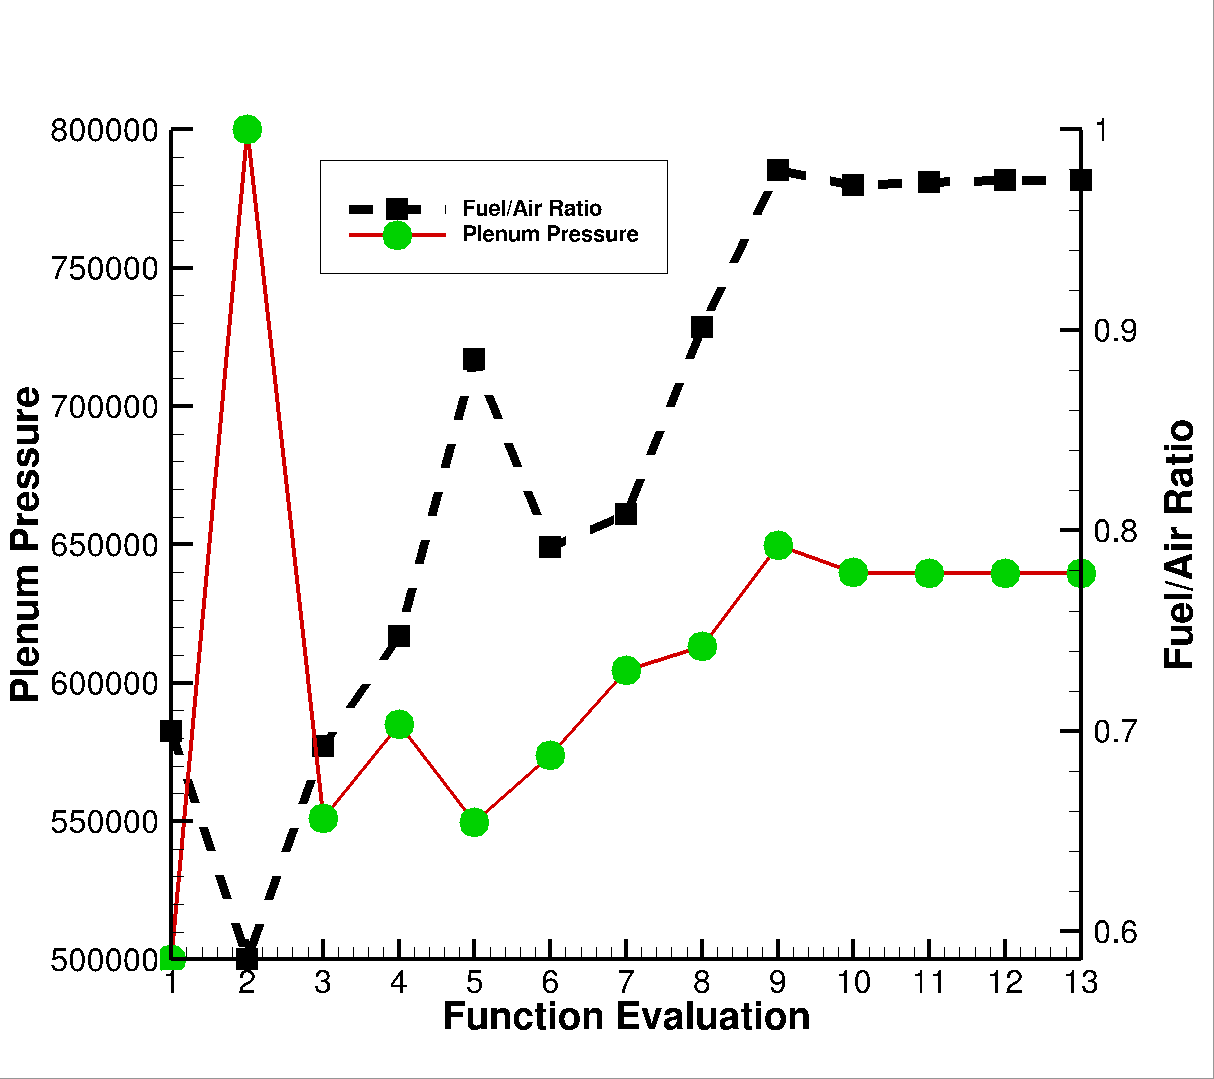
\includegraphics[width=\textwidth]{figures/1st-H2/dv_hist.png}
    \caption{Design Variable History}
    \label{fig:dv-hist-1st-H2}
  \end{subfigure}
  \begin{subfigure}[b]{0.45\textwidth}
    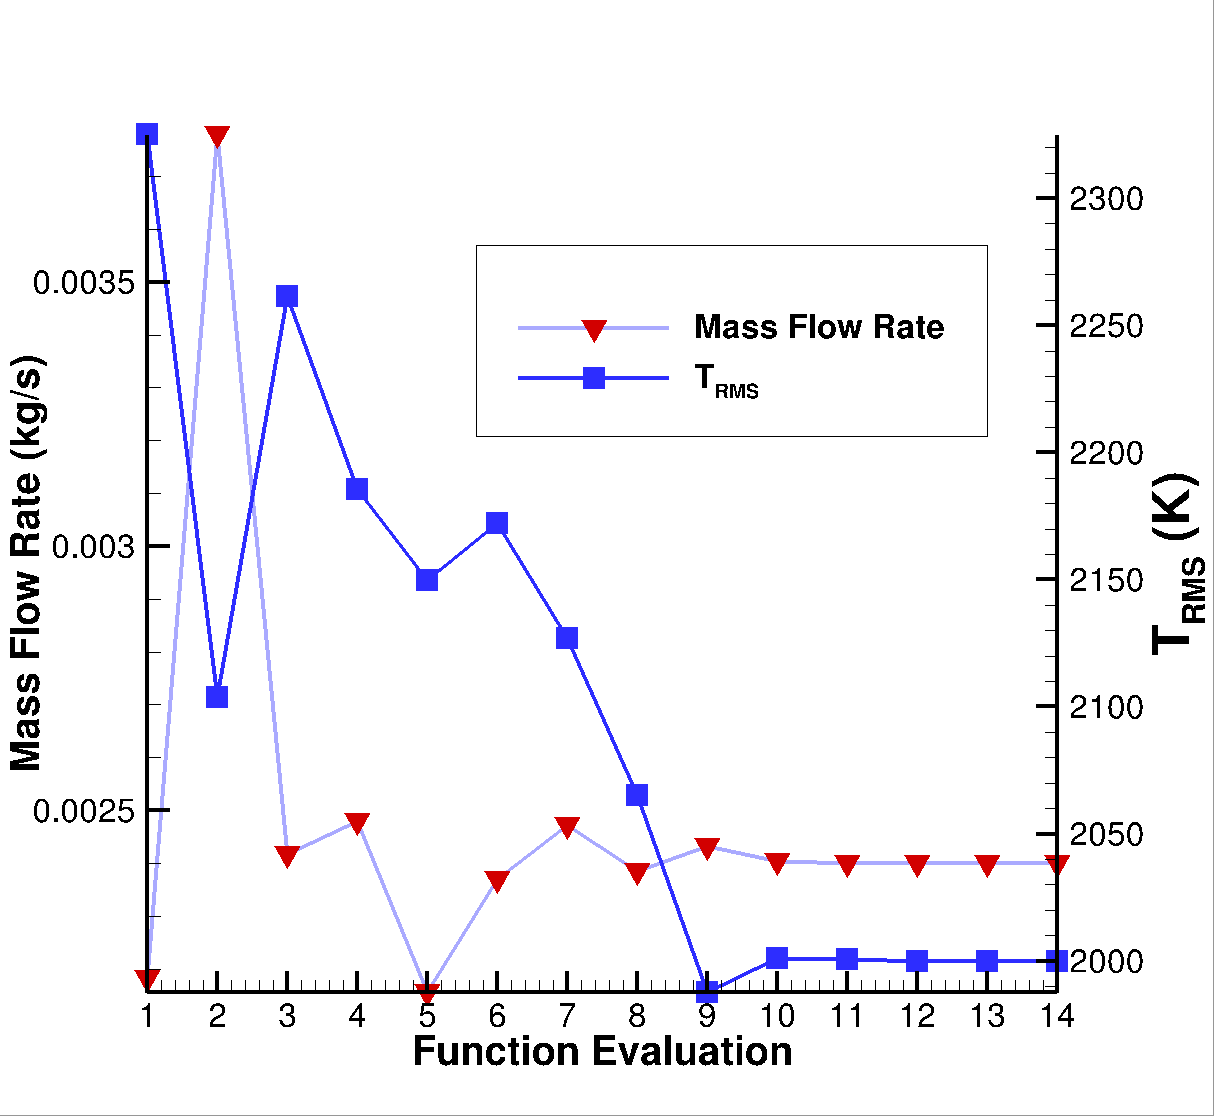
\includegraphics[width=\textwidth]{figures/1st-H2/fm_hist.png}
    \caption{Design Variable History}
    \label{fig:fm-hist-1st-H2}
  \end{subfigure}
  \caption{Inverse Design History}
\end{figure}
%------------------------------------------------------------------------------%
Using the SNOPT optimizer, \fref{fig:cost-func-1st-H2} shows that the target
design was met within 13 function evaluations.  SNOPT explores the entire design
space, as is show in the second function evaluation, where a spike in the cost
function occurred.
\fref{fig:dv-hist-1st-H2} indicates that the optimizer tried the upper
bound for the plenum pressure design variable, and found that sensitivity
derivatives indicated that the lower pressure was required. This is common, and
is an effective way to insure that there is a local minimum in the prescribed
bound.  The optimization terminated when the cost function value was less than
the tolerance of $10^{-8}$, and \fref{fig:components-1st-H2} shows that both
components of the cost function were within one order of magnitude of each other
during the optimization.  This last point is important, since non-normalized
components can skew the optimization results, where competing components can
cause oscillations in the function evaluations and stall the optimization
procedure.  \fref{fig:fm-hist-1st-H2} shows the history of the surface
temperature RMS and annular nozzle mass flow rate, with the design targets.  The
optimization clearly made significant progress early, with smaller gains as the
solution approached the target.

\section{Direct Design Optimization}

Using the same cost function components and design variables as in
\sref{inv-design-opt}, a direct design problem was completed to minimize both
mass flow rate and surface temperature RMS.  The cost function was formulated as
%------------------------------------------------------------------------------%
\begin{equation}
  f = w_1\left( \massflow \right)^2 + w_2\left( T_{RMS} \right)^2
  \label{direct-design-cost-func}
\end{equation}
%------------------------------------------------------------------------------%
With the weights chosen in the same manner as the inverse design problem to
insure that the components are normalized to the same order of magnitude
%------------------------------------------------------------------------------%
\begin{equation}
  \frac{w_1}{w_2} = \frac{\left( \massflow \right)^2}{\left( T_{RMS} \right)^2}
  \label{direct-design-weights}
\end{equation}
%------------------------------------------------------------------------------%
The SNOPT optimizer was able to very quickly determine that blowing pure
$H_2$, i.e. $\fa = 1.0$, would yield the lowest surface temperature RMS and mass
flow rate.  \fref{fig:dd-cost-func-value} shows that most of the improvement in
the design was made within the first two function evaluations, and the
subsequent steps were significantly less.
%------------------------------------------------------------------------------%
\begin{figure}[h]
  \centering
	\begin{subfigure}[b]{0.4\textwidth}
    \centering
    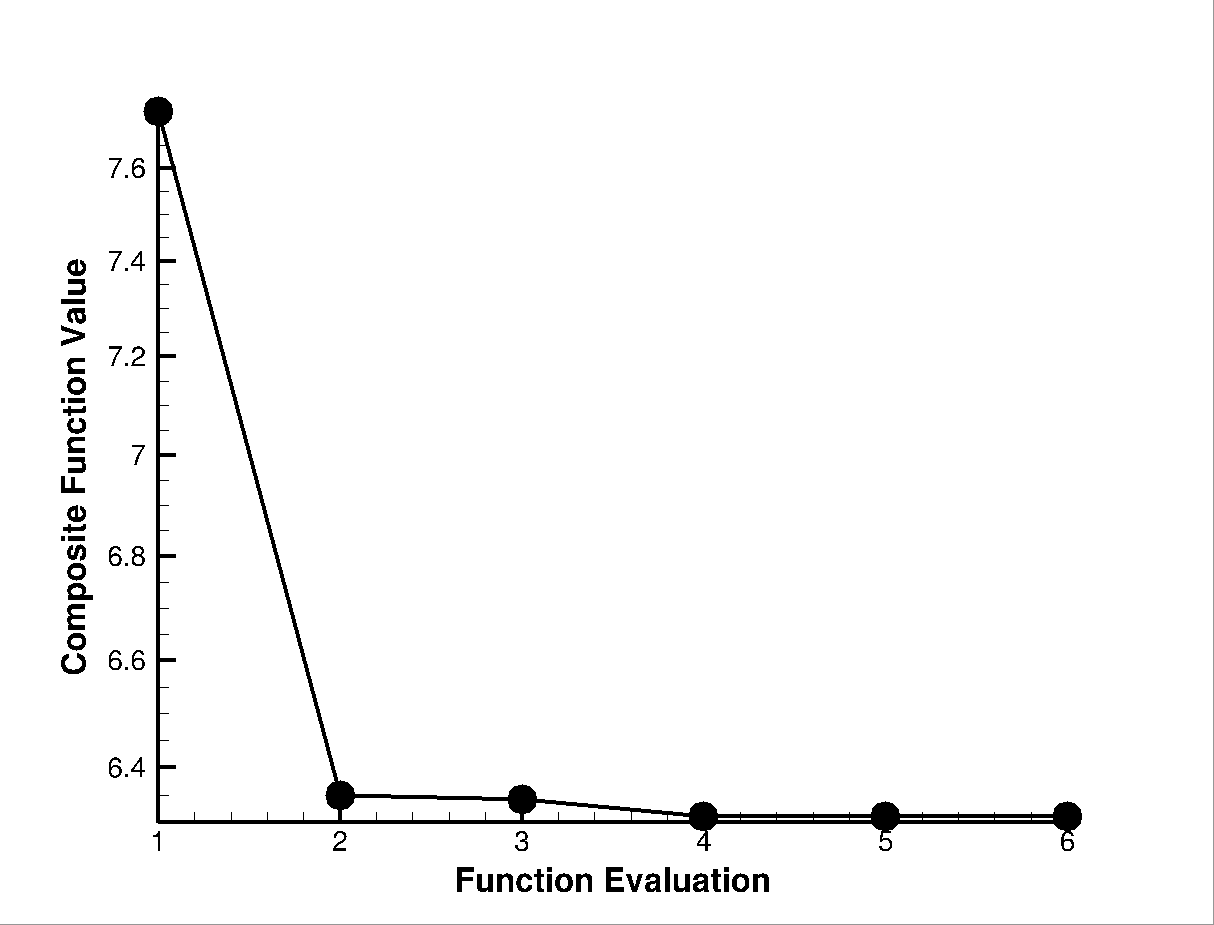
\includegraphics[width=\textwidth]{figures/direct_design/cost-func.png}
    \caption{Composite Cost Function Value}
    \label{fig:dd-cost-func-value}
  \end{subfigure}
	\begin{subfigure}[b]{0.4\textwidth}
    \centering
    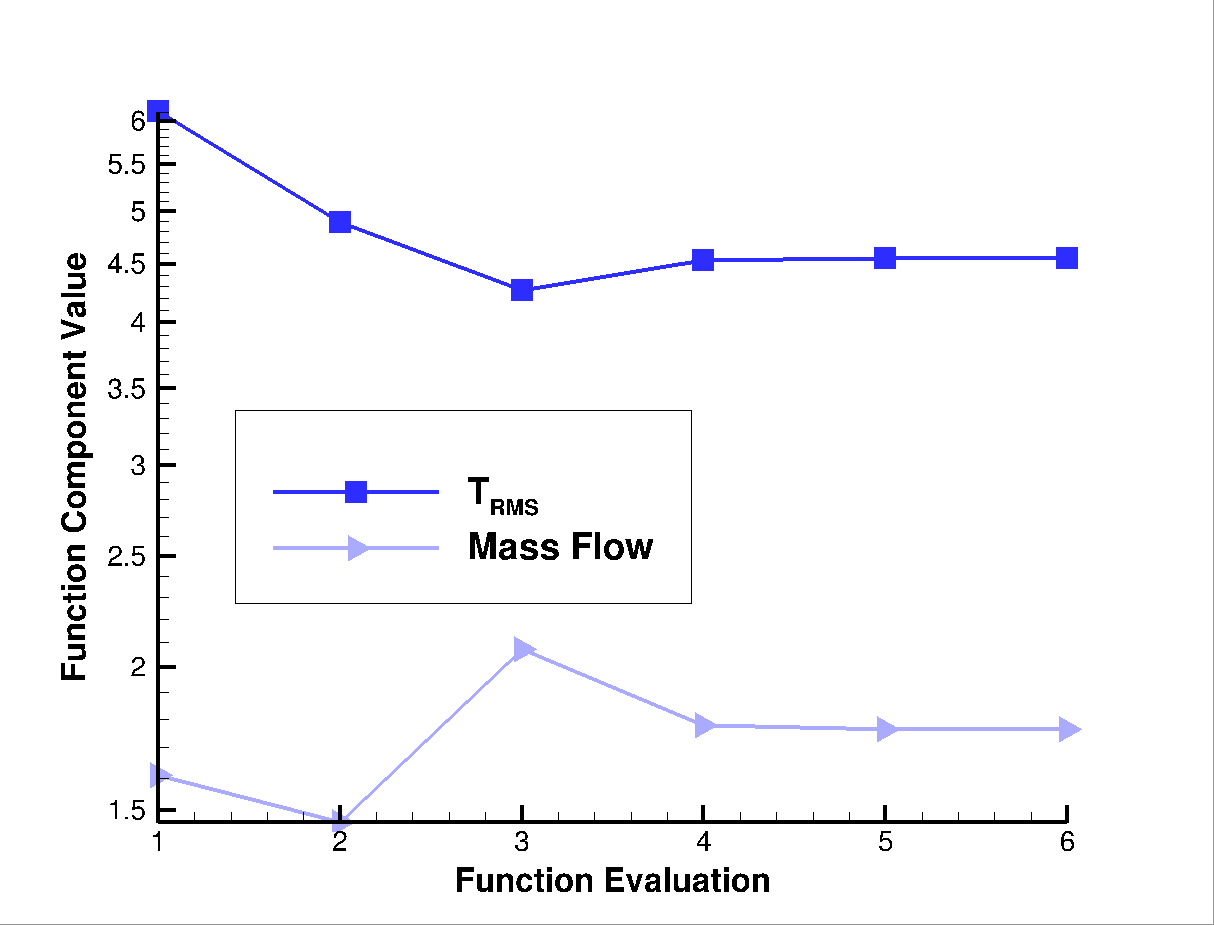
\includegraphics[width=\textwidth]{figures/direct_design/components.png}
    \caption{Cost Function Components}
    \label{fig:dd-components}
  \end{subfigure}
  \caption{Direct Design Cost Function}
  \label{fig:dd-cost-func}
\end{figure}
%------------------------------------------------------------------------------%
\fref{fig:dd-components} verifies that weights determined by
\eref{direct-design-weights} were indeed sufficient to normalize $\massflow$ and
$T_{RMS}$ contributions to the composite cost function.
%------------------------------------------------------------------------------%
\begin{figure}[h]
  \centering
	\begin{subfigure}[b]{0.4\textwidth}
    \centering
    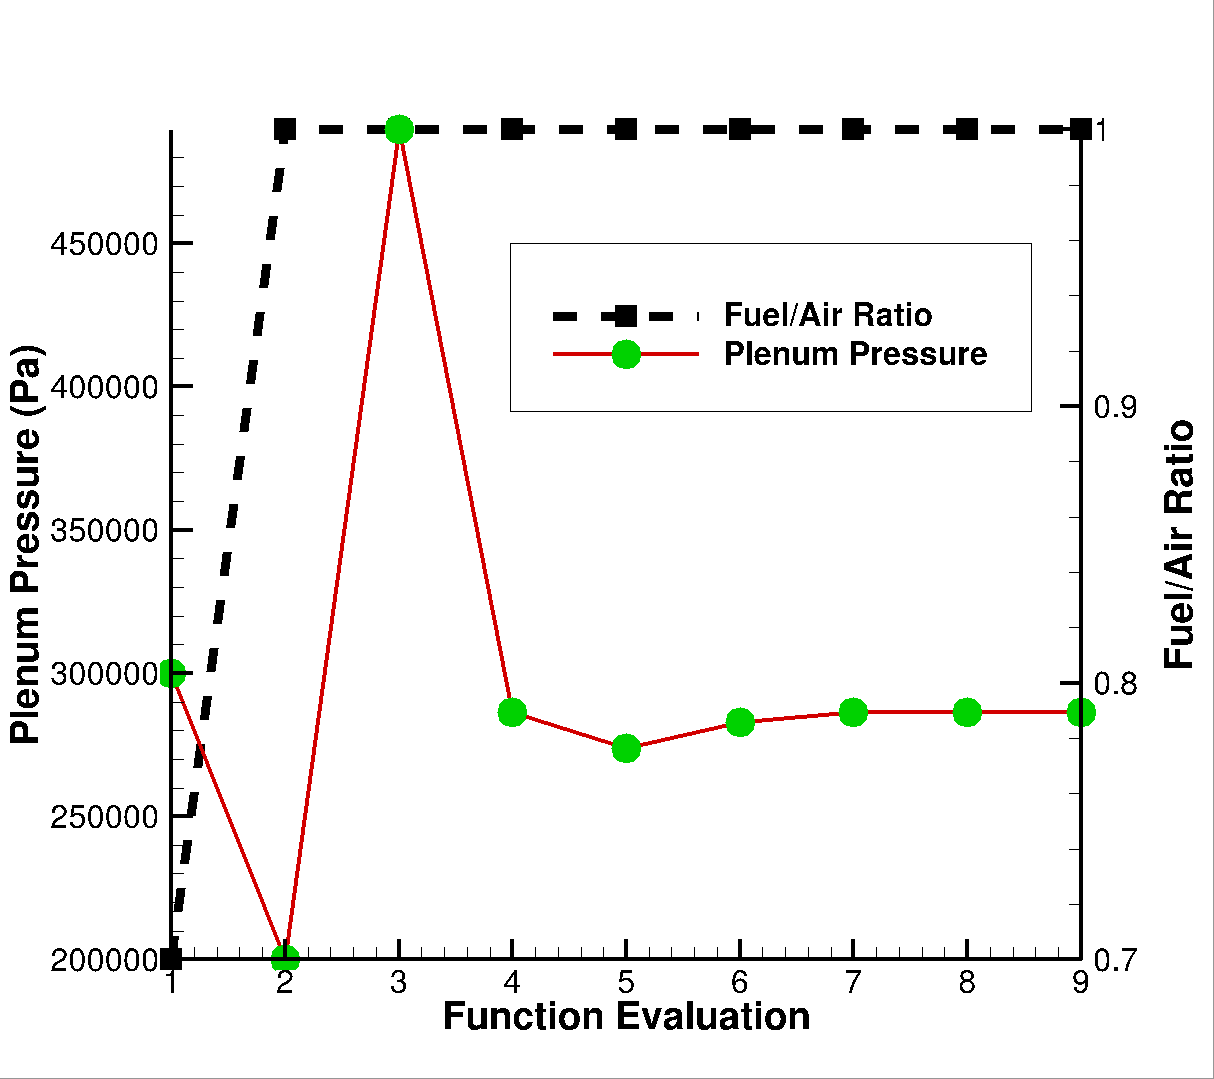
\includegraphics[width=\textwidth]{figures/direct_design/dv-hist.png}
    \caption{Design Variable History}
    \label{fig:dd-dv-hist}
  \end{subfigure}
	\begin{subfigure}[b]{0.4\textwidth}
    \centering
    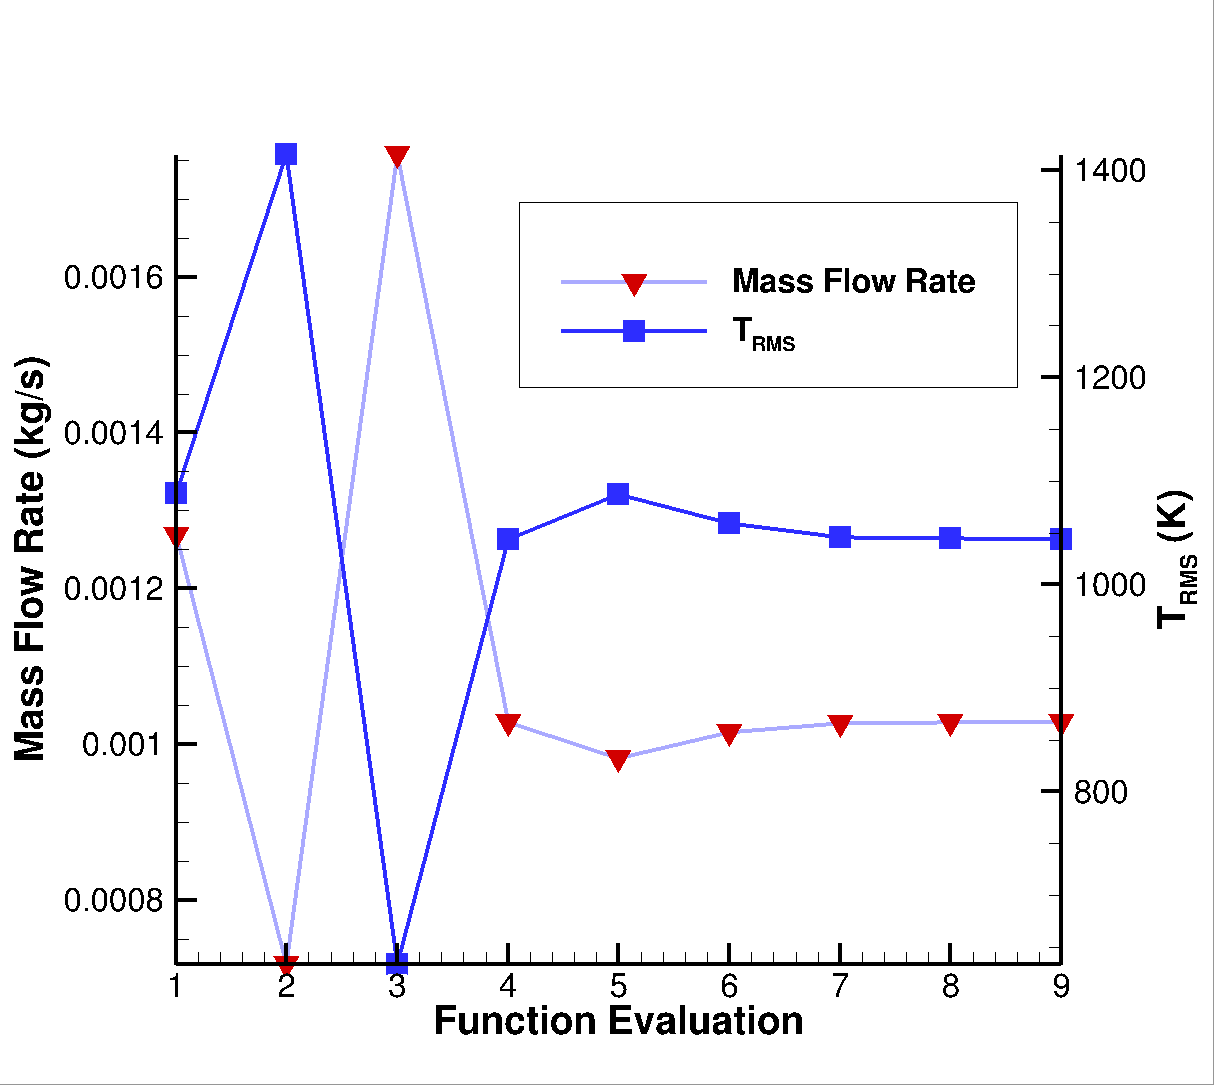
\includegraphics[width=\textwidth]{figures/direct_design/mass-tt.png}
    \caption{$\massflow$ and $T_{RMS}$ Design History}
    \label{fig:dd-mass-tt}
  \end{subfigure}
  \caption{Direct Design History}
  \label{fig:dd-history}
\end{figure}
%------------------------------------------------------------------------------%
\fref{fig:dd-dv-hist} shows that the optimization was largely dependent on the
plenum pressure, and \tref{tab:design-improvement} shows that larger pressure at
the plenum resulted in a 13.79\% lower surface temperature, at the expense of a
4.6\% higher mass flow rate.
%------------------------------------------------------------------------------%
\begin{table}[h]
  \centering
  \begin{tabular}{c|c|c|c}
    Component & Initial & Final & Improvement\\
    \hline
    $\dot{m}$, $kg/s$ & 1.268e-3 & 1.327e-3 & -4.6\% \\
    $T_{RMS}$, $K$    & 2473     & 2132     & 13.79\%
  \end{tabular}
  \caption{Direct Design Optimization Improvement}
  \label{tab:design-improvement}
\end{table}
%------------------------------------------------------------------------------%
This is an excellent problem for a high-fidelity gradient-based
optimization, as the non-linear effects of plenum-shock interation makes the
optimum plenum condition difficult to determine intuitively.

There is a much stronger dependence on the choice of cost function weights for
this problem than for the inverse design problem in \sref{inv-design-opt}.  For
the inverse design problem, the target mass flow rate and surface temperature
RMS were known a priori; therefore, the weighting was chosen as a purely
normalizing measure to accelerate convergence to the target condition.  For this
direct design problem the target mass flow rate and surface temperature RMS are
not know a priori, and the weights chosen have a direct impact on the optimum
condition.  A ``skewed'' weighting may be advisable from an engineering
perspective when attempting a direct design approach.  For example, if the
surface thermal protection (TPS) is rated to withstand much higher surface
heating than what is nominally predicted, a higher weight might be given to the
mass flow rate in order to decreased the required vehicle mass.  The heuristic
nature of this approach can be avoided by setting a component target, or
converting a composite cost function component to an explicit constraint.  The
latter option is more robust, but comes at the cost of an additional adjoint
solution.
